\documentclass[border=4pt]{standalone}
% Shared TikZ preamble for book diagrams
% Usage: % Shared TikZ preamble for book diagrams
% Usage: % Shared TikZ preamble for book diagrams
% Usage: \input{../preamble.tex} after \documentclass

\usepackage{tikz}
\usepackage{amsmath,amssymb}

\usetikzlibrary{arrows.meta, calc, positioning, decorations.pathreplacing}

% --- Color palette ---
% Consistent across all diagrams in the book
\definecolor{basis1}{RGB}{31,119,180}    % blue: encoders, structure
\definecolor{msg}{RGB}{44,160,44}        % green: positives
\definecolor{aux}{RGB}{127,127,127}      % gray: alternatives, auxiliary
\definecolor{highlight}{RGB}{255,127,14} % orange: highlights
\definecolor{lightfill}{RGB}{230,240,255}% light blue: shaded regions

% --- Reusable styles ---
\tikzset{
  encoder/.style={draw=basis1!60, fill=lightfill, rounded corners=3pt,
    minimum width=1.0cm, minimum height=0.8cm},
  flow/.style={-{Stealth[length=5pt,width=4pt]}, line width=0.8pt},
  annotation/.style={font=\footnotesize, text=aux!80!black},
}
 after \documentclass

\usepackage{tikz}
\usepackage{amsmath,amssymb}

\usetikzlibrary{arrows.meta, calc, positioning, decorations.pathreplacing}

% --- Color palette ---
% Consistent across all diagrams in the book
\definecolor{basis1}{RGB}{31,119,180}    % blue: encoders, structure
\definecolor{msg}{RGB}{44,160,44}        % green: positives
\definecolor{aux}{RGB}{127,127,127}      % gray: alternatives, auxiliary
\definecolor{highlight}{RGB}{255,127,14} % orange: highlights
\definecolor{lightfill}{RGB}{230,240,255}% light blue: shaded regions

% --- Reusable styles ---
\tikzset{
  encoder/.style={draw=basis1!60, fill=lightfill, rounded corners=3pt,
    minimum width=1.0cm, minimum height=0.8cm},
  flow/.style={-{Stealth[length=5pt,width=4pt]}, line width=0.8pt},
  annotation/.style={font=\footnotesize, text=aux!80!black},
}
 after \documentclass

\usepackage{tikz}
\usepackage{amsmath,amssymb}

\usetikzlibrary{arrows.meta, calc, positioning, decorations.pathreplacing}

% --- Color palette ---
% Consistent across all diagrams in the book
\definecolor{basis1}{RGB}{31,119,180}    % blue: encoders, structure
\definecolor{msg}{RGB}{44,160,44}        % green: positives
\definecolor{aux}{RGB}{127,127,127}      % gray: alternatives, auxiliary
\definecolor{highlight}{RGB}{255,127,14} % orange: highlights
\definecolor{lightfill}{RGB}{230,240,255}% light blue: shaded regions

% --- Reusable styles ---
\tikzset{
  encoder/.style={draw=basis1!60, fill=lightfill, rounded corners=3pt,
    minimum width=1.0cm, minimum height=0.8cm},
  flow/.style={-{Stealth[length=5pt,width=4pt]}, line width=0.8pt},
  annotation/.style={font=\footnotesize, text=aux!80!black},
}

\begin{document}
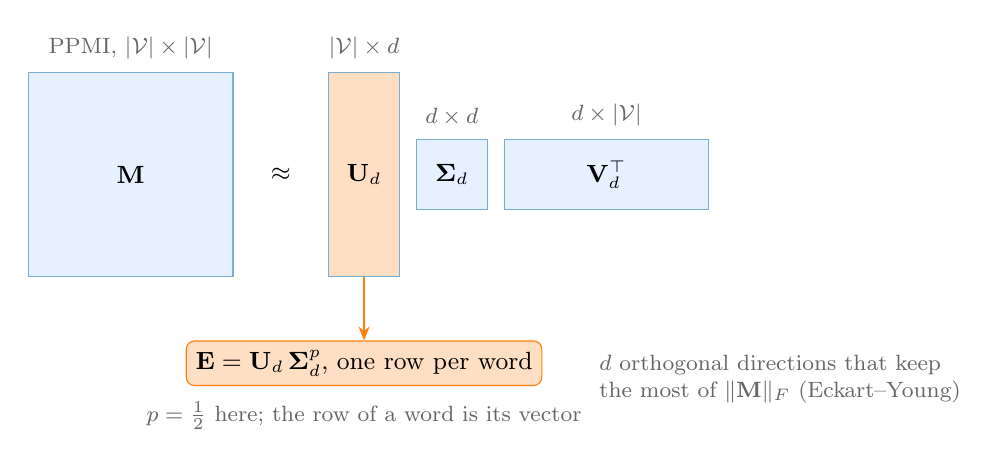
\begin{tikzpicture}[font=\small]
  % PPMI matrix M (V x V) ~ U_d Sigma_d V_d^T
  \node[draw=basis1!60, fill=lightfill, minimum width=2.6cm, minimum height=2.6cm] (M) {$\mathbf{M}$};
  \node[annotation, above=1pt of M] {PPMI, $|\mathcal{V}|\times|\mathcal{V}|$};
  \node[right=0.35cm of M] (approx) {$\approx$};
  \node[draw=basis1!60, fill=highlight!25, minimum width=0.9cm, minimum height=2.6cm, right=0.35cm of approx] (U) {$\mathbf{U}_d$};
  \node[annotation, above=1pt of U] {$|\mathcal{V}|\times d$};
  \node[draw=basis1!60, fill=lightfill, minimum width=0.9cm, minimum height=0.9cm, right=0.2cm of U] (S) {$\mathbf{\Sigma}_d$};
  \node[annotation, above=1pt of S] {$d\times d$};
  \node[draw=basis1!60, fill=lightfill, minimum width=2.6cm, minimum height=0.9cm, right=0.2cm of S] (Vt) {$\mathbf{V}_d^{\top}$};
  \node[annotation, above=1pt of Vt] {$d\times|\mathcal{V}|$};
  % embedding
  \draw[flow, highlight] (U.south) -- ++(0,-0.8) coordinate (a);
  \node[draw=highlight, fill=highlight!25, rounded corners=3pt, below=0.8cm of U, minimum width=3.4cm] (E) {$\mathbf{E}=\mathbf{U}_d\,\mathbf{\Sigma}_d^{p}$, one row per word};
  \node[annotation, below=2pt of E] {$p=\tfrac12$ here; the row of a word is its vector};
  % geometry
  \node[annotation, anchor=west, align=left] at ([xshift=0.6cm,yshift=-0.2cm]E.east)
    {$d$ orthogonal directions that keep\\the most of $\lVert\mathbf{M}\rVert_F$ (Eckart--Young)};
\end{tikzpicture}
\end{document}
